\documentclass[10pt,twocolumn,letterpaper]{article}

\usepackage{iccv}
\usepackage{times}
\usepackage{epsfig}
% \usepackage{graphicx}
\usepackage{amsmath}
\usepackage{amssymb}
\usepackage[activate]{pdfcprot}
\usepackage{xcolor}
\usepackage[color]{changebar}

% Include other packages here, before hyperref.

% for figures and captions
\usepackage{graphicx}
\usepackage{subcaption}
\graphicspath{{figs/}}

% in-paragraph enumerate
\usepackage{paralist}

% better citing
\usepackage[numbers,square]{natbib}

% If you comment hyperref and then uncomment it, you should delete
% egpaper.aux before re-running latex.  (Or just hit 'q' on the first latex
% run, let it finish, and you should be clear).
\usepackage[pagebackref=true,breaklinks=true,colorlinks,bookmarks=false]{hyperref}

% temporarily uncommented as reverse-search wasn't working for me
% it looks like the hacked-together iccv.sty broke something with the synctex
\iccvfinalcopy % *** Uncomment this line for the final submission

\def\iccvPaperID{1113} % *** Enter the ICCV Paper ID here
\def\httilde{\mbox{\tt\raisebox{-.5ex}{\symbol{126}}}}

\cbcolor{red}
\newcommand{\todo}[1]{\cbstart \textsf{\textbf{\textcolor{red}{[#1]}}} \cbend{}}
\newcommand{\commentE}[1]{\textsf{\textbf{\textcolor{green}{Erroll: #1}}}}
\newcommand{\commentA}[1]{\textsf{\textbf{\textcolor{orange}{Andreas: #1}}}}
\newcommand{\commentT}[1]{\textsf{\textbf{\textcolor{blue}{Tadas: #1}}}}
\newcommand{\commentY}[1]{\textsf{\textbf{\textcolor{yellow}{Yusuke: #1}}}}

% create a command to set dataset name
\newcommand{\dataset}{SynthesEyes\xspace}

% Pages are numbered in submission mode, and unnumbered in camera-ready
\ificcvfinal\pagestyle{empty}\fi
\begin{document}

%%%%%%%%% TITLE
% \title{Photorealistic Rendering of Face and Eye Regions for Eyelid Detection and Gaze Estimation}
\title{Learning-by-Synthesis: Photorealistic Rendering of Eyes for Eye Registration and Gaze Estimation}
% Erroll: we'd like to replace "eyelid detection" with something a bit more descriptive, as our system loacalizes them accurately and also gives estimates for iris and therefore eye-centre also. Perhaps "Eye Registration?"
% \title{Photorealistic Rendering of Human Eyes for Eyelid Detection and Gaze Estimation}
% Andreas; learning-by-synthesis we could also use in the title
% Andreas: what about "Photorealistic Rendering of Face and Eye Images for Large-Scale Eyelid Detection and Gaze Estimation" 

\author{removed\\
for\\
{\tt\small blind review}
% For a paper whose authors are all at the same institution,
% omit the following lines up until the closing ``}''.
% Additional authors and addresses can be added with ``\and'',
% just like the second author.
% To save space, use either the email address or home page, not both
% \and
% Second Author\\
% Institution2\\
% {\tt\small secondauthor@i2.org}
}

\maketitle
%\thispagestyle{empty}

%%%%%%%%% ABSTRACT
\begin{abstract}
%!TEX root = syntheyes15.tex

High-quality images of the human eye are required in the study of several computer vision problems, such as facial feature detection and tracking, eye detection, or gaze estimation and correction.
In particular recent large-scale supervised methods require tedious and time-consuming collection and typically manual annotation of large amounts of training images.
%, which is error-prone and slows down progress in these areas.
We present a novel method to synthesise photorealistic close-up images of the human eye for arbitrary head poses, gaze directions, and lighting conditions.
At the core of our method is a dynamic eye-region model that we \todo{briefly describe what this model involves and how it was generated}
The model is able to simulate the large variability of real eyes, including pupil dilation, eyelid motion and corresponding changes in its shape, as well as iris colour variations.
%dynamic changes in shape
We demonstrate the usefulness of our method on the sample problems of eyelid detection and appearance-based gaze estimation.
We show that \todo{results}
\end{abstract}

%%%%%%%%% BODY TEXT


\section{Introduction}


\section{Related work}

%!TEX root = syntheyes15.tex

\section{Our dynamic eye-region model}

\begin{figure*}
    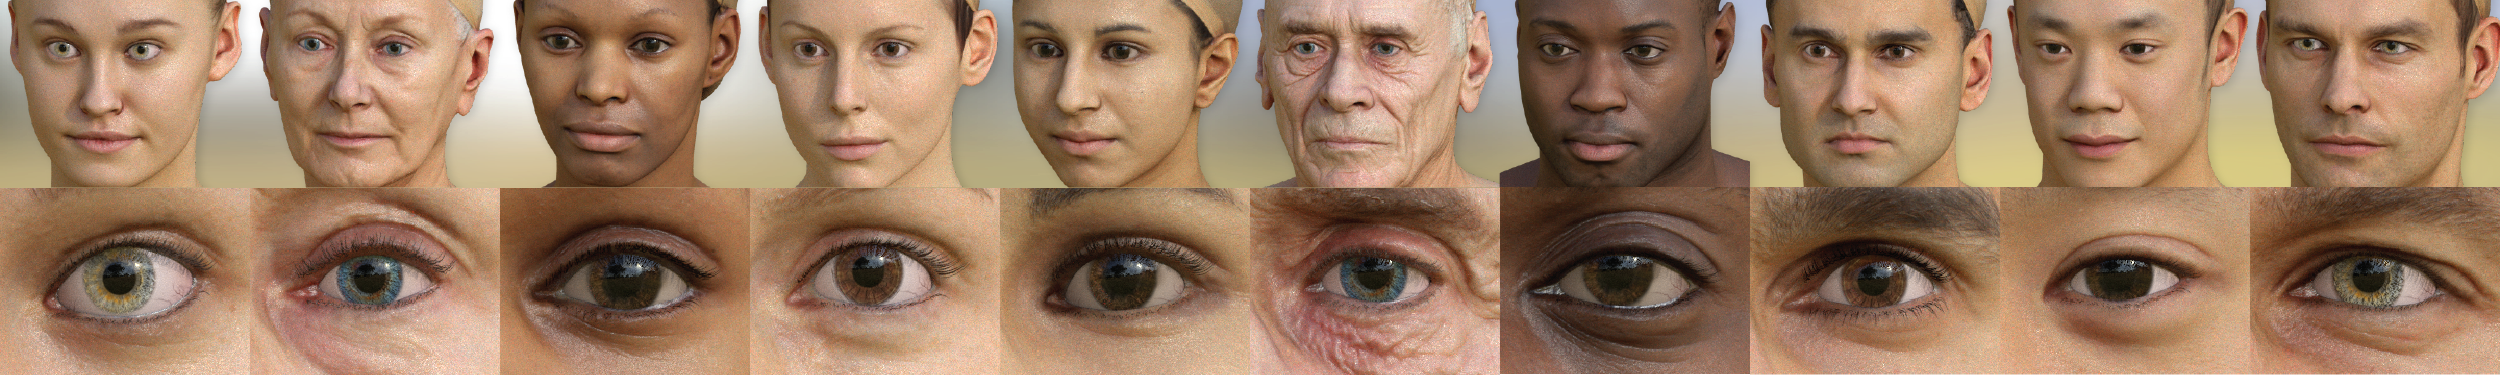
\includegraphics[width=\textwidth]{model_suite}
    \caption{Set of head models and corresponding close-ups of the eye regions used in our method. The set includes 10 different head models of both genders that cover a range of ethnicities and ages.}
    \label{fig:model_suite}
\end{figure*}

In this section we first present our anatomically inspired CG eyeball model, and then explain our novel procedure for preparing a suite of 3D head scans for dynamic photorealistic labelled data generation.

% \cite{MIL-STD-1472G} -- cite for range of eye rotation.

\subsection{Reduced eyeball model}
\label{subsec:eyeball_model}

\begin{figure}
    \centering
    \begin{subfigure}[t]{0.33\columnwidth}
        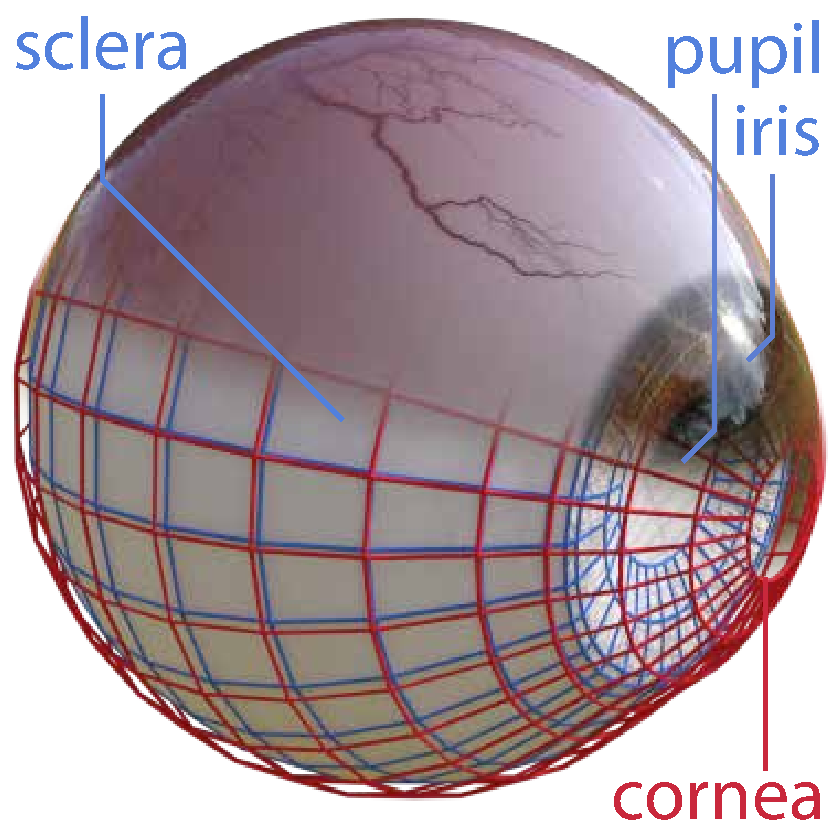
\includegraphics[width=\textwidth]{eye_model}
        \caption{3D eye model}
        \label{fig:3d_eye_model}
    \end{subfigure}%
    \hfill
    \begin{subfigure}[t]{0.65\columnwidth}
        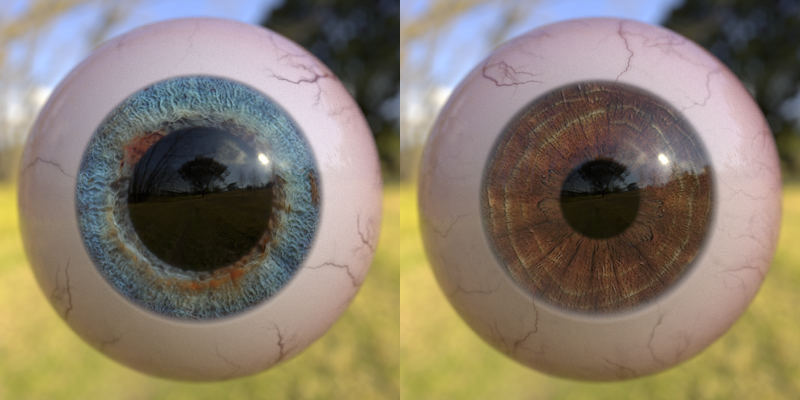
\includegraphics[width=\textwidth]{eye_examples}
        \caption{Pupil dilation and iris color variation}
    \end{subfigure}
    \caption{Our realistic eye model is capable of expressing degrees of variability seen in real life.}
    \label{fig:eye_model}
\end{figure}

Eyeballs are complex organs comprised of multiple layers of tissue, each with different reflectance properties and levels of transparency. Fortunately, as realistic eyes are so important for many areas of CG, there is already a large body of previous work on modelling and rendering eyes \commentE{cite}.

% It is important to accurately model reflections and refractions in the eye as they can lead to specular highlights -- these common eye-region image features are often used by eye-tracking algorithms, or can confound approaches that are not robust.

As shown in \autoref{fig:3d_eye_model}, our eye model consists of two parts.
%
The outer part (red wireframe) approximates the eye's overall shape with two spheres ($r_1\!=\!12\textrm{mm}, r_2\!=\!8\textrm{mm}$ \cite{ruhland2014look}), the latter representing the corneal bulge. To avoid a discontinuous seam between spheres, the meshes were joined and then smoothed. It is transparent, refractive ($n\!=\!1.376$), and partially reflective. The eye's bumpy surface variation is modelled by a displacement map generated with noise functions.
%
The inner part (blue wireframe) is a flattened sphere with Lambertian material. The planar end represents the iris and pupil, and the rest represents the sclera -- the white of the eye.
%
There is a $0.5\textrm{mm}$ gap between the outer and inner parts which accounts for the thickness of the cornea. \commentE{compare with recent Disney work}

Eyes exhibit variations in both shape (pupillary dilation) and texture (iris color and scleral veins). To model shape variation we use \emph{shape keys} -- a CG animation technique where different versions of a mesh are stored, modified, and interpolated between \cite{orvalho2012facial}. \commentE{more on shape keys} We have shape keys representing dilated and constricted pupils, as well as large and small irises to account for a small amount ($10\%$) of variation in iris size.

We vary the appearance of the eye by compositing textures in three separate layers:
\begin{inparaenum}[\itshape i\upshape)]
\item a \emph{sclera} layer representing the tint of the sclera (white, pink, or yellow);
\item an \emph{iris} layer with four photo-textures of different colored irises (amber, blue, brown, grey); and
\item a \emph{veins} layer which varies between blood-shot and clear
\end{inparaenum}. We matched the sclera tint to each separate face model, but uniformably randomly varied iris color. Previous research on iris-synthesis \commentE{cite} would have allowed continually different iris textures, but we decided this added complexity would not make a worthwhile improvement in overall appearance variation, especially when rendered at lower resolutions.

\subsection{3D head scan acquisition}

\begin{figure*}
    \centering
    \begin{subfigure}[t]{0.195\textwidth}
        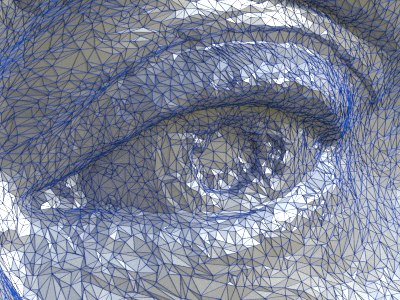
\includegraphics[width=\textwidth]{process_f02_01}
        \caption{Original 3D head scan data: 1.4 million polys}
        \label{fig:process_original_scan}
    \end{subfigure}
    \hfill
    \begin{subfigure}[t]{0.195\textwidth}
        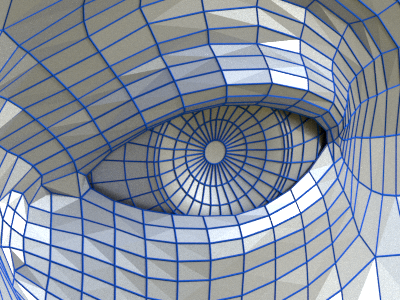
\includegraphics[width=\textwidth]{process_f02_02}
        \caption{Retopologized head model: 9 thousand polys}
        \label{fig:process_retopo}
    \end{subfigure}
    \hfill
    \begin{subfigure}[t]{0.195\textwidth}
        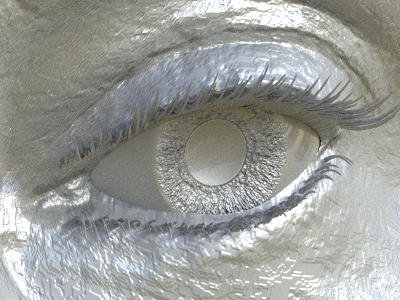
\includegraphics[width=\textwidth]{process_f02_03}
        \caption{Surface detail is stored in displacement maps}
        \label{fig:process_displaced_subdiv}
    \end{subfigure}
    \hfill
    \begin{subfigure}[t]{0.195\textwidth}
        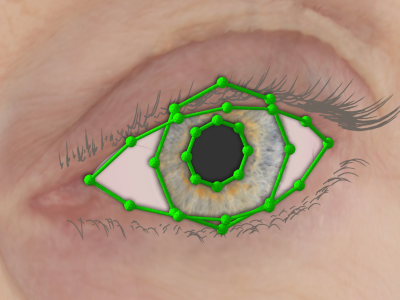
\includegraphics[width=\textwidth]{process_f02_04}
        \caption{3D iris and eyelid landmarks are annotated}
    \end{subfigure}
    \hfill
    \begin{subfigure}[t]{0.195\textwidth}
        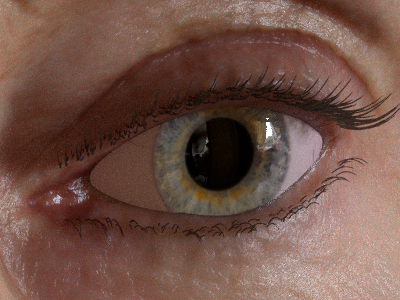
\includegraphics[width=\textwidth]{process_f02_05}
        \caption{The final render}
    \end{subfigure}
    \caption{Model preparation process}
    \label{fig:process}
\end{figure*}

Photogrammetry is becoming a popular ...

We start with high quality production-level scans purchased from a photogrammetry studio's online store.

\subsection{Eye-region geometry preparation}

As can be seen in \autoref{fig:process_original_scan}, the cornea has been incorrectly reconstructed in the head scan. This is because transparent surfaces are not directly visible, so cannot be reconstructed in the same way as diffuse surfaces like skin. Recent work uses a hybrid reconstruction method to reconstruct the corneal surface seprately, but requires additional hardware \cite{berard2014highquality} -- this level of detail was deemed unneccesary for our purposes. We want to render eye-region images representing a wide range of eye-gaze directions, so we need to be able to pose the eyeball separately from the face geometry. We therefore remove the scanned eyeball from the mesh using boolean operations, and place our own eyeball approximation (\autoref{subsec:eyeball_model}) in its place.

While the original head scan geometry is suitable for being rendered as a static model, its topology cannot easily represent dynamic changes in eye-region shape. Vertical saccades are always accompanied by eyelid motion \cite{liversedge2011oxford}, so we need to be able to pose the eyelids according to the gaze vector. When preparing a mesh for facial animation, edge loops should flow along and around the natural contours of facial muscles. This leads to a more efficient (lower-resolution) geometric representation of the face, and more realistic animation as mesh deformation mathes that of actual muscles.

We therefore \emph{retopologize} the face geometry into a more optimal form using a commercial semi-automatic system \cite{ZRemesher}. \commentE{Reference some other options, e.g automatic methods in research} As can be seen in \autoref{fig:process_retopo}, edge loops now follow the \emph{Orbicularis Oculi} muscle, allowing for realistic eye-region deformations. This retopologized low-poly mesh lacks the detail of the original scan (e.g. the crease above the eye), and has visible sharp edges. We therefore use it as the control mesh for a displaced subdivision surface \cite{lee2000displaced}, with displacement map computed from the scanned geometry. As can be seen in \autoref{fig:process_displaced_subdiv}, skin surface detail like wrinkles and creases is  restored.

Although they are two seperate organs, there is normally no visible gap between eyeball and skin. However, as a consequence of removing the eyeball from the original scan, the retopologized mesh will not necessarily meet the geometry of our eyeball model (\autoref{fig:process_retopo}). To compensate, the face mesh's eyelid vertices are displaced along their normals to their respective closest positions on the eyeball geometry (\autoref{fig:process_displaced_subdiv}). This automatic operation ensures the models are joined, even after changes in pose \cite{Shrinkwrap}.

\subsection{Eyelashes}

Eyelashes are short curved hairs that grow from the outer edges of the eyelids. These can occlude parts of the eye and affect eye-tracking algorithms, so should be simulated. We follow the approach of \citet{swirski2014rendering}, and model them using directed hair particle effects. The hair particles are generated from a smoothed control surface below the eyelid edges and directed away from the face. To make them curl, the eyelash particles experience a slight amount of gravity during growth (negative gravity for the upper eyelash).

\subsection{Eyelid motion}

Create face, eyelash, and landmark blend shapes for eyelids looking up and down.

\begin{figure}
    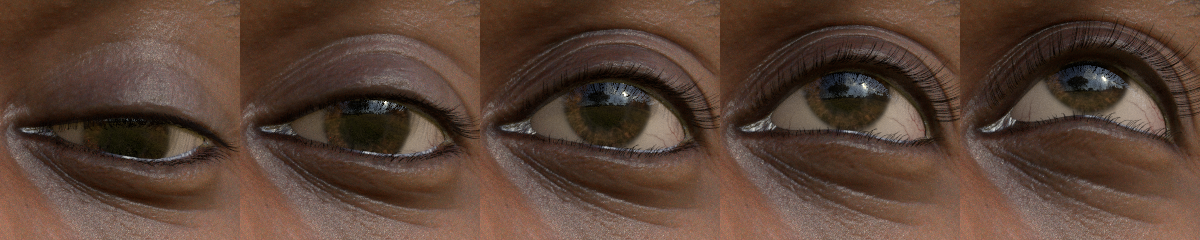
\includegraphics[width=\columnwidth]{eyelid_motion.png}
    \caption{Eyelids are posed using blend shapes linked to the gaze vector. Note how we use wrinkle-maps to simulate the folding of the skin above and below the eye.}
\end{figure}
%!TEX root = syntheyes15.tex

\section{Rendering photo-realistic training images}

We briefly describe how we use image-based lighting \cite{debevec2002image} to model a wide range of realistic lighting conditions, and finally discuss the details of our rendering setup.

\begin{figure}
    \centering
    \begin{subfigure}[t]{0.48\columnwidth}
        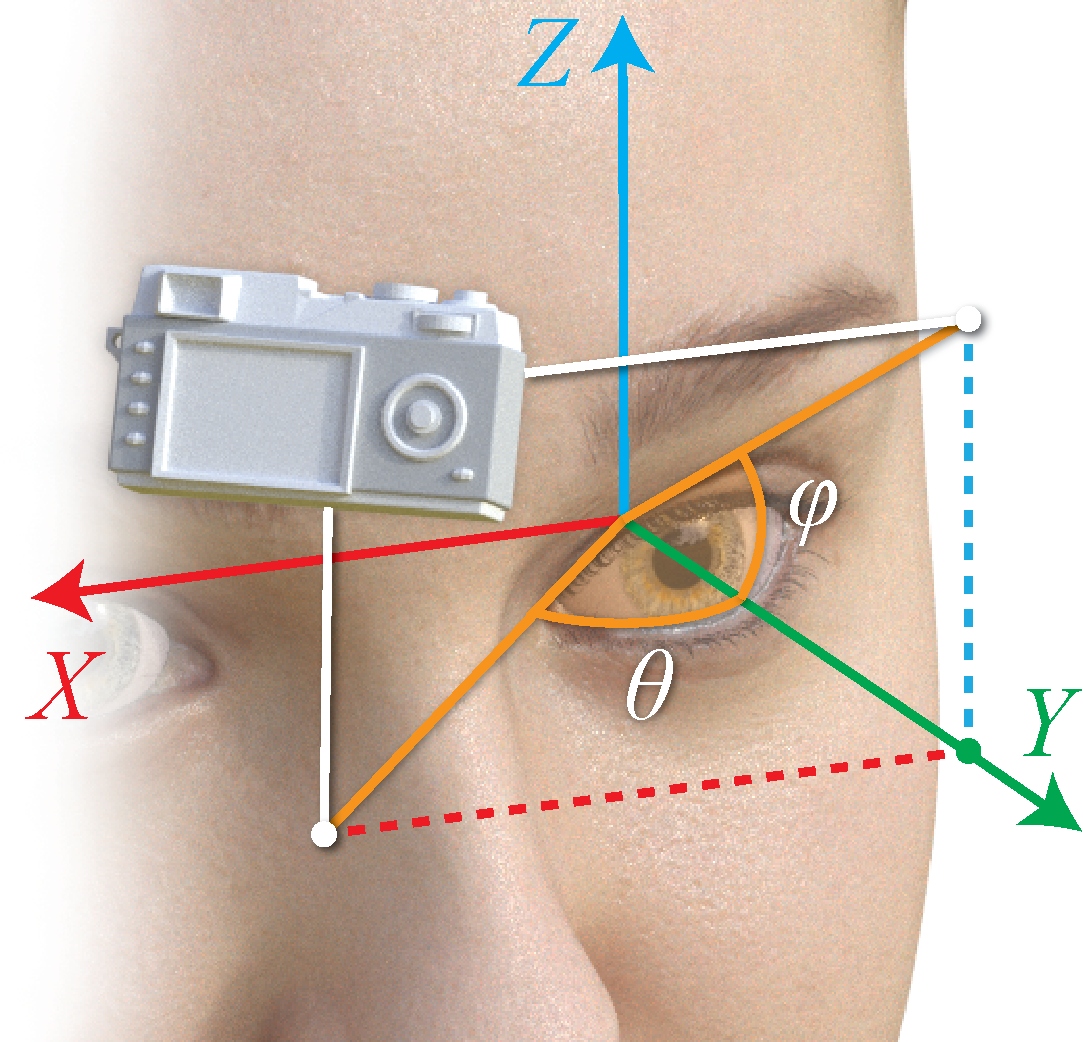
\includegraphics[width=\textwidth]{camera_position}
        \caption{The camera is positioned using spherical coordinates}
        \label{fig:cam_pos_spher_coords}
    \end{subfigure}
    \hfill
    \begin{subfigure}[t]{0.48\columnwidth}
        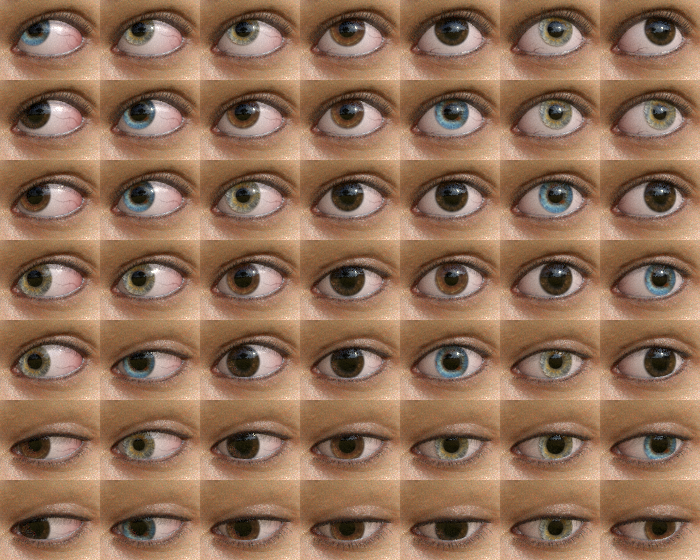
\includegraphics[width=\textwidth]{camera_pos_sample_renders_7x7}
        \caption{Example renderings from one camera position}
        \label{fig:cam_pos_example_renders}
    \end{subfigure}
    \caption{\ref{fig:cam_pos_spher_coords} shows how we position the camera to simulate changes in head pose. At each camera position, we render many eye images (\ref{fig:cam_pos_example_renders}) by posing the eyeball model.}
\end{figure}

\subsection{Lighting}

\begin{figure}
    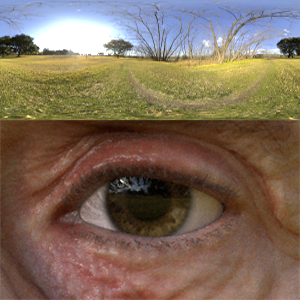
\includegraphics[width=0.24\columnwidth]{fig_env_1} \hfill
    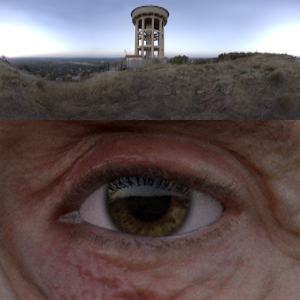
\includegraphics[width=0.24\columnwidth]{fig_env_2} \hfill
    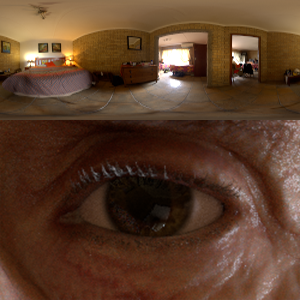
\includegraphics[width=0.24\columnwidth]{fig_env_3} \hfill
    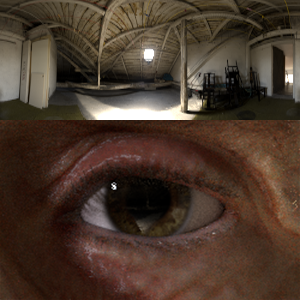
\includegraphics[width=0.24\columnwidth]{fig_env_4}
    \caption{Appearance variation from lighting is modelled with poseable high-dynamic-range environment maps \cite{debevec2002image}.}
    \label{fig:participants}
\end{figure}

\subsection{Computational setup}

We can rapidly generate diverse datasets much faster than manual collection and annotation.
%!TEX root = syntheyes15.tex

\section{Experiments}

We evaluated the usefulness of our method on two sample problems, namely eyelid detection and gaze estimation.
\commentA{briefly say something about significance/importance of both problems, more in corresponding subsections}

\subsection{Eyelid Detection}

\commentA{results look pretty good already, I suggest put them in asap so that we can completely draft this subsection. If results improve we can always update later but this way we have something to produce text and refine the story}

\begin{itemize}
    \item Evaluate eyelid landmark accuracy on LFW and M-PIE data, compare against several state-of-the-art CLM methods.
    \item Evaluate eyelid and iris landmarks on hand-annotated MPII data, compare against a baseline method: majority vote for iris position.
\end{itemize}

% show that we only need data from few(er) people and show competitive performance
(Maybe) Plot landmark accuracy on LFW against number of training participants. Show that even with just a few participants (e.g. 4) we get good results for eyelid positions compared to state-of-the-art face trackers.

% eye corner detection
% eye bounding box detection
% eye position detection?
% ^ I think all of these come with what the deformable model gives us

\subsection{Gaze Estimation}

% evaluate eye/gaze/eyelid shapes (fully synthetic) separately from full face appearance (which is a mixture of real and synthetic data)

% person-adaptation, use pre-trained model from synthesised data, then personalise with small amount of user-specific data
% ^ let's leave this as future work! Can put it in the discussion 

% show that we can synthesise specific datasets for specific settings (specific head and gaze ranges, illumination conditions), show that we can competitive performance
We render a targeted dataset that matches MPII's gaze and pose distribution, with added 3D laptop screen emitting light. This shows how we can target specific scenarios like laptop-based gaze estimation, and render a suitable dataset within a day rather than take 3 months of data collection.

% train on synthesised images and show competitive performance on MPIIgaze with real images
% show better performance than UT dataset
Using Xucong's CNN sytem, we train on targeted version of \dataset, test on MPII. Show results are better than training on UT and testing on MPII. This shows that the range of lighting in \dataset is important for better results.

% does photorealistic data really help/is it necessary? either reduce quality and see how it affects performance, or compare model with and without shape variations
% ^ I am not really sure how to do this well... Because we'd also have to have a measure of "how photorealistic" something is. Swapping the eyeball for a simpler model, e.g. sphere might not really have that much of an effect on "photorealism" for many eye-poses. Changing the shaders, e.g. pretending the skin is Lambertian (diffuse) might?



\section{Conclusion}


{\small
\bibliographystyle{IEEEtranN}
\bibliography{bib}
}

\end{document}
